\chapter{Complex variables and vector spaces}
\minitoc
\pagebreak
\section{Complex Numbers revision}
\subsection{Basics}
We start with a basic revision of complex numbers.
 Complex numbers were initially introduced to ensure that every polynomial of degree n has n roots. 
 A complex number, $z$, can be expressed in 3 forms:
\begin{enumerate}
	\item $z=x+iy$
	\item $z=R(cos\theta+isin\theta)$
	\item $z=Re^{i\theta}$
\end{enumerate}
In case your memory is that poor, $i$ is the square root of -1.
 Addition of complex numbers is defined as follows $$(x+iy) + (a+ib) = (x+a) + i(y+b) $$
which should be pretty obvious.
 Subtraction is not defined explicitly but by changing $a$ to $-a$ and $b$ to $-b$.
  Multiplication is also defined $$(x+iy)(a+ib) = (ax-by)+i(bx+ay)$$
\subsection{Argand Diagrams}
An argand diagram is a way of representing a complex number on a 2D plane.
 The real component of $z$ is plotted on the x-axis whilst the imaginary component is plotted on the y-axis.
 %
 \begin{minipage}[t]{0.47\linewidth}
 	\begin{figure}[H]
 		\centering
 		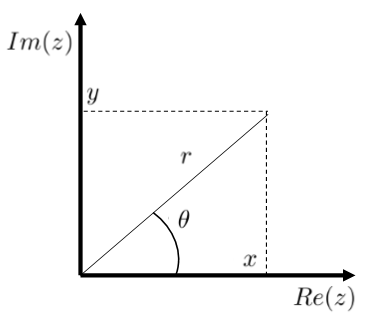
\includegraphics[width=\linewidth]{complex/argand}
 		\captionsetup{font=small} 	
 	\end{figure} 
 \end{minipage}
 \hspace{0.6cm}
%
\begin{minipage}[t]{0.47\linewidth}
	\vspace{1cm}
	We can define the modulus 
	%
	\begin{align*}
	\mid z \mid &= \sqrt{x^2+y^2} \\
	&= (x+iy)(x-iy) \\
	&= z\overline{z}.
	\end{align*}
	%
	In addition to this, $\theta$ is often referred to as the argument.
	 Note that the argument is not unique, you can add $2\pi$ to the argument and obtain the same result, so it's often useful to think of the principal value argument adding the contraint that $\theta$ lies between $0$ and $2\pi$
\end{minipage}
\begin{examples}
	We'll start with a few basic examples to refresh your memory, given $z_1=1+i$ \& $z_2=2+3i$:
	\begin{enumerate}
		\item Find the cube root of $z_1$
		\item Find the modulus and argument of $z_1z_2$
	\end{enumerate}
\textbf{Answers:} 1. $2^{1/6}exp(\frac{\pi}{12})$, $2^{1/6}exp(\frac{3\pi}{4})$, $2^{1/6}exp(\frac{17\pi}{12})$ \hspace{0.5cm}
2. $\mid z\mid = \sqrt{26}$, $arg(z)=1.77$
\end{examples}
\subsection{Mappings}
If we have a complex function $w=f(z)$, then you can think of this function as a mapping from the domain, the $z$ complex plane to the co-domain, the $w$ complex plane.